\begin{titlepage}
    \centering
    \vspace*{\fill}

    \vspace*{0.5cm}

    \Large% \bfseries
    Análise de longo prazo (1985 – 2018) das mudanças florestais na Mata Atlântica utilizando o algoritmo Landtrendr

    \vspace*{5cm}

    % \large Eduardo Ribeiro Lacerda

    \vspace*{\fill}
\end{titlepage}

\section{Análise de longo prazo (1985 – 2018) das mudanças florestais na Mata Atlântica utilizando o algoritmo Landtrendr}

\begin{abstract}
    abstract
\end{abstract}

% Os resultados obtidos mostram uma Mata Atlântica com concentrações de perda na parte sul e nordeste do pais, e com ganhos locais distribuídos por todo o bioma. A Mata Atlântica que foi desmatada e fragmentada ao longos dos séculos se vê hoje ganhando mais do que perdendo em área total, mas as perdas e os ganhos não podem ser tratados de forma igualitária. A perda fere mais a saúde do bioma por interferir majoritariamente em áreas antigas e bem estruturadas, enquanto os ganhos, por serem eventos ainda recentes, são frágeis e não possuem a mesma resiliência. 

\subsection{Introdução}
\hspace{13pt} Estamos na década da restauração (2020 - 2030), e o desafio para alcançar as metas são enormes. A Mata Atlântica, como uma das regiões mais biodiversas do mundo \citep{REZENDE2018208}, tem papel importante nesse desafio. Movimentos como a criação do Pacto pela Mata Atlântica em 2009 visando a restauração de 15 Mha de áreas degradadas até 2050, servem para mostrar a importância que o bioma tem para a conservação da parte considerável da biodiversidade mundial com suas quase 16 mil espécies de plantas e mais de 2 mil espécies de vertebrados.  



\subsection{Resultados para os eventos de perda na Mata Atlântica}
\hspace{13pt} Somando-se todos os eventos de perda detectados pelo algoritmo após as filtragens das áreas de interesse, houveram ao longo de todos os anos da análise 61.167.796 de pixels com uma perda média de magnitude de 225 ou diminuição de 0.225 no índice NDVI. Isso equivale a uma área total de pouco mais de 55 mil $ km^2 $ de florestas que sofreram perdas significativas no bioma e que não foram recuperadas após a supressão.

O resultado mais abrangente envolvendo todos os eventos de perda do bioma pode ser visualizado na (Figura \ref{fig:heat_loss_masked85_maskedgain}). A maior aglomeração de eventos de perda está localizada principalmente entre os estados do Paraná e Santa Catarina e no estado da Bahia. Nos outros estados o mapa de calor mostra uma distribuição mais homogênea dos eventos ao longo do território. 

\begin{figure}[H]
    \centering
    \includegraphics[scale=.5]{images/heatmap_loss_masked85_maskedgain.pdf}
    \caption{Todos os eventos de perda na Mata Atlântica entre 1985 e 2018.}
    \label{fig:heat_loss_masked85_maskedgain}
\end{figure}

Quando a divisão das detecções é feita de acordo com eventos de curta duração (um ano) e longos (maiores que um ano), verificamos que o padrão espacial das aglomerações (\textit{clusters}) se mantém semelhante com apenas algumas variações (Figura \ref{fig:heat_loss_eq1_neq1}). Os eventos de curta duração tendem a se localizar mais na fronteira entre Paraná e Santa Catarina, enquanto os de longa aconteceram com maior frequência na região central do Paraná, sul/norte da Bahia e norte de Pernambuco. Dos mais de 61 milhões de eventos detectados ou 55 mil $ km^2 $, cerca de 27.5 milhões foram eventos de curta duração, o que significa uma área aproximada de 25 mil $ km^2 $. Os outros 33.7 milhões de eventos tiveram duração maior que um ano, o que totalizou aproximadamente 30.4 mil $ km^2 $.

Já quando a divisão é feita por estados (Figura \ref{fig:estados_loss_masked85_maskedgain}), verificamos que estados como Minas Gerais possuem um número grande de eventos que estão distribuídos de forma homogênea pelo território, assim como Bahia e São Paulo. Vemos que apesar do maior \textit{cluster} de perdas estar localizado entre Paraná e Santa Catarina, a maior quantidade de eventos está no estado do Paraná. 

\begin{figure}[H]
    \centering
    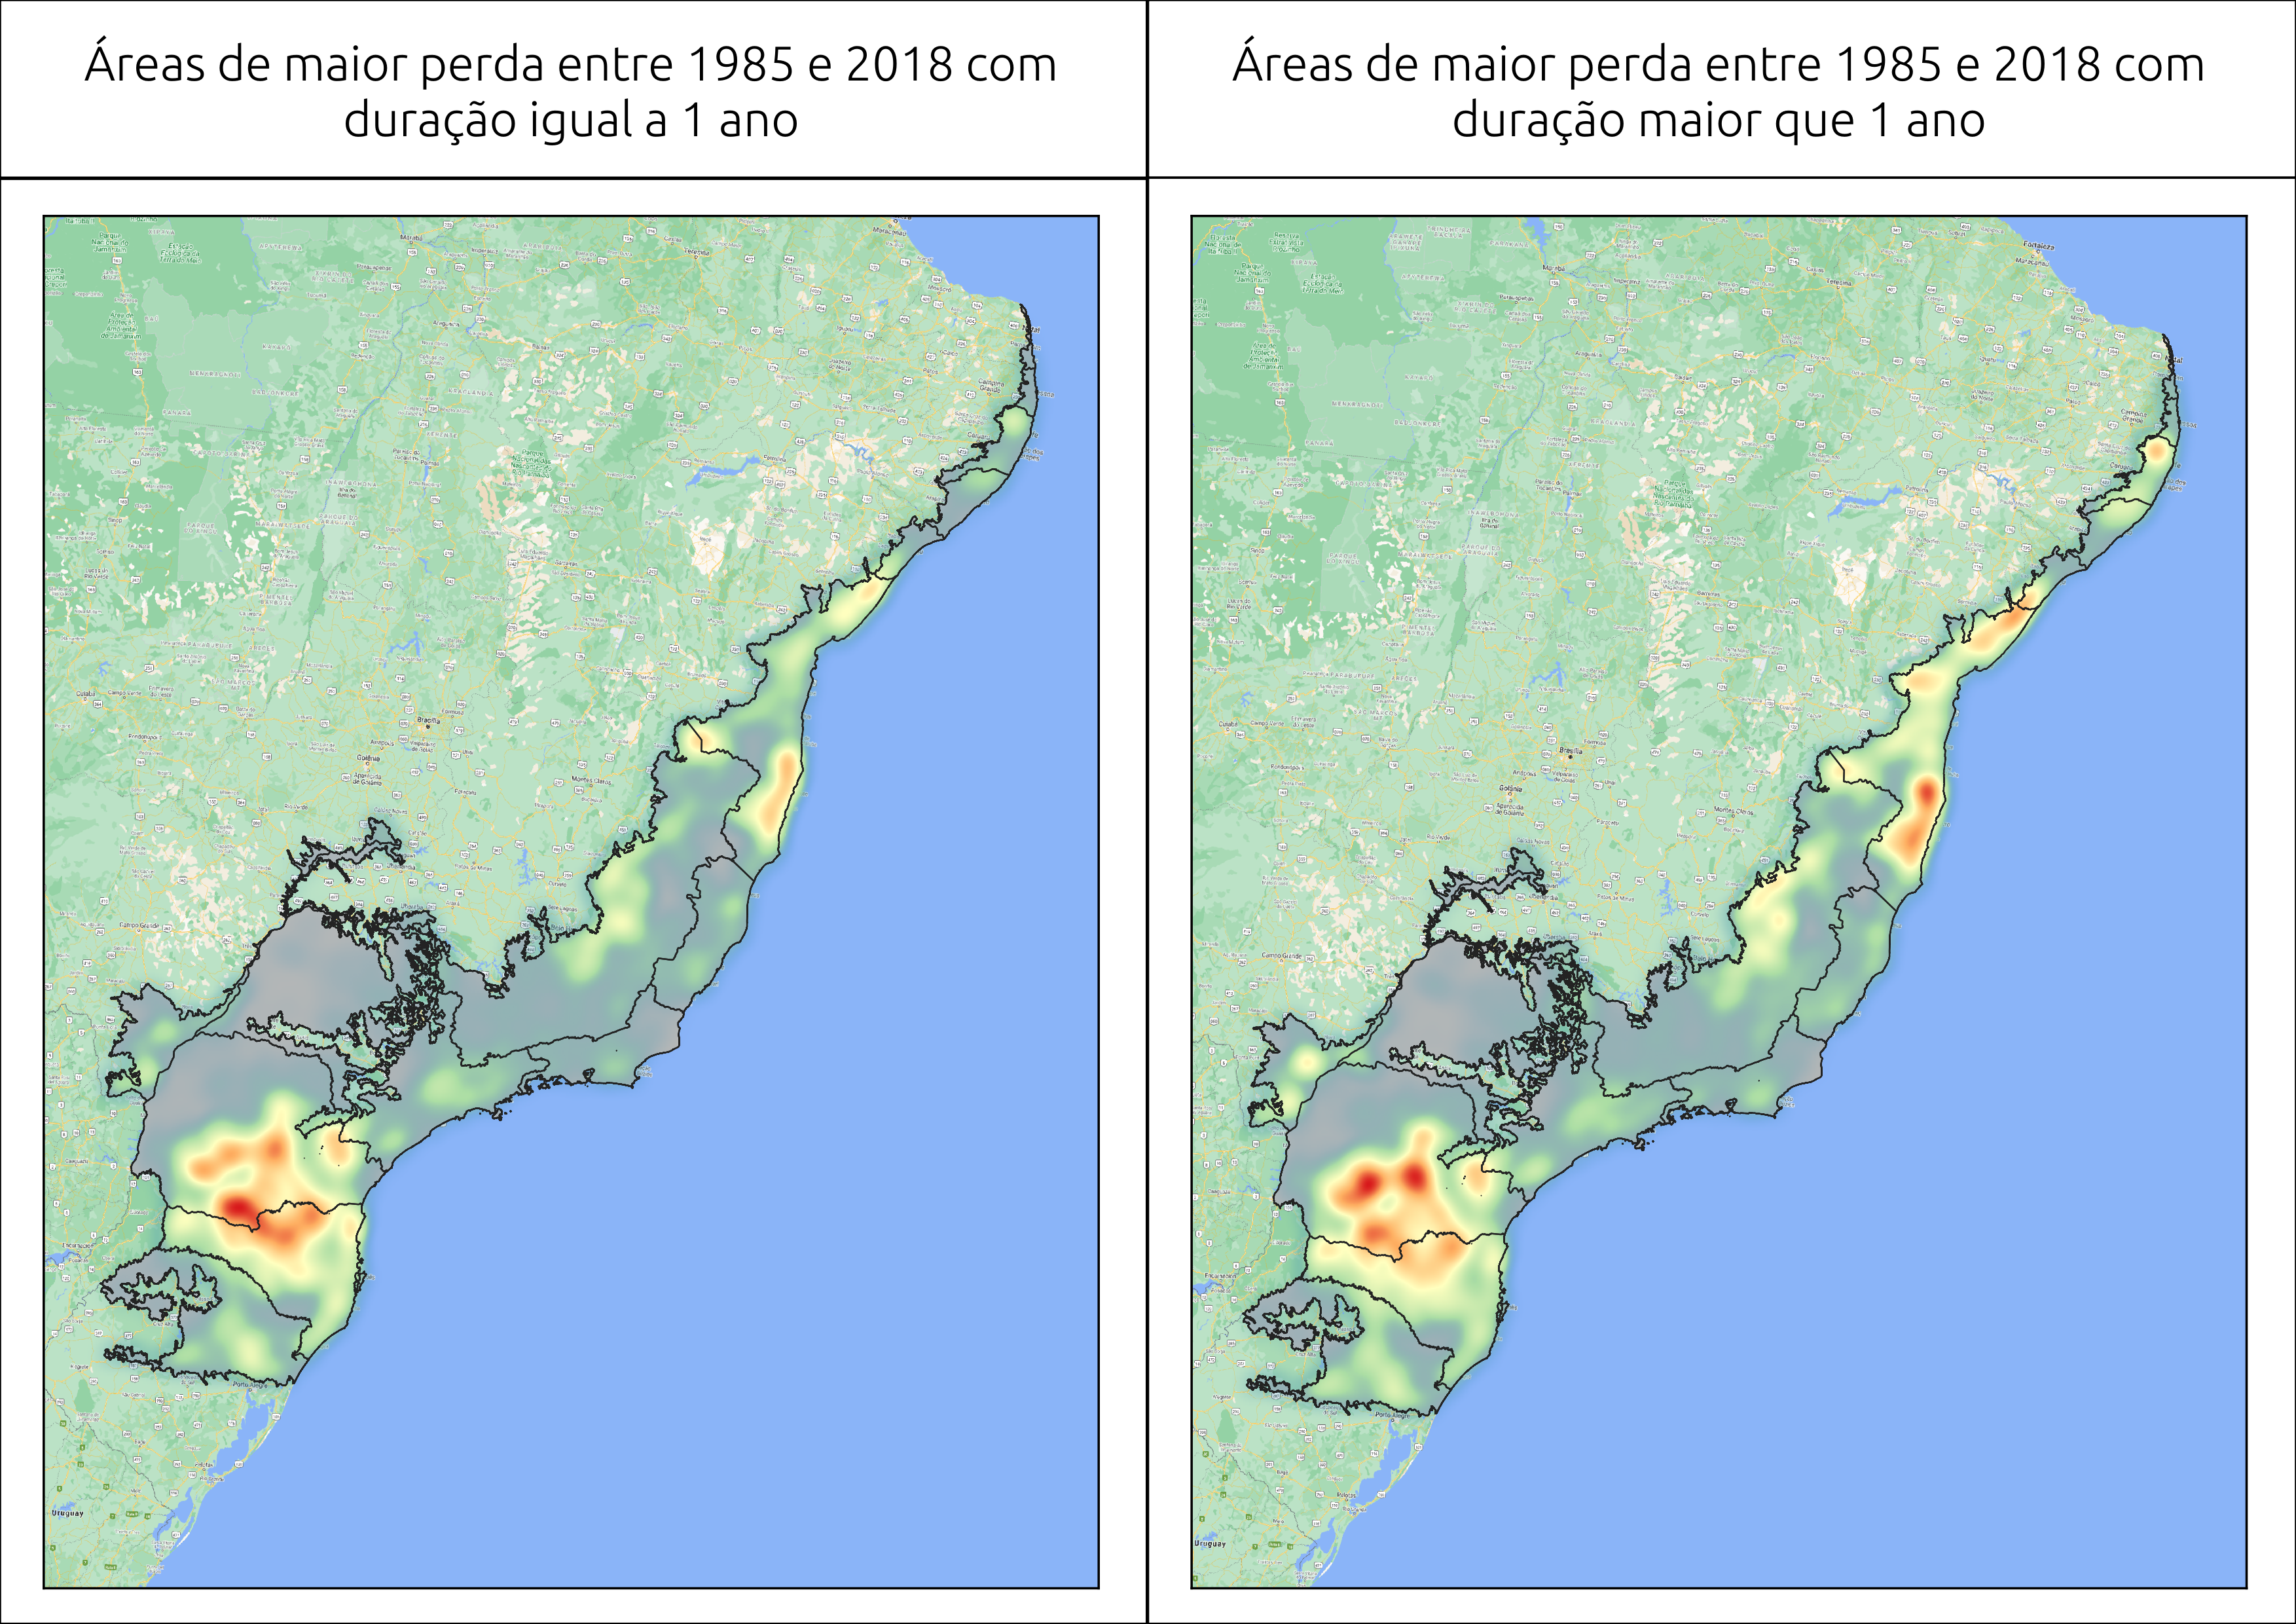
\includegraphics[scale=.5]{images/heatmap_loss_eq1_neq1.pdf}
    \caption{Mapas com os eventos de perda entre 1985 e 2018 tanto com duração igual a 1 quanto somente maiores que 1.}
    \label{fig:heat_loss_eq1_neq1}
\end{figure}

\begin{figure}[H]
    \centering
    \includegraphics[scale=.5]{images/estados_loss_masked85_maskedGain.pdf}
    \caption{Todos os eventos de perda na Mata Atlântica entre 1985 e 2018 por estado. Os valores representam o número de pixels que tiveram alguma detecção de perda.}
    \label{fig:estados_loss_masked85_maskedgain}
\end{figure}

Ao considerar o número de eventos de acordo com a área de cada estado, verificamos que estados como Santa Catarina e Bahia se destacam mostrando o maior proporção de perdas ao longo dos 33 anos seguido de Pernambuco, Paraná e Sergipe (Figura \ref{fig:estados_loss_proporcional}).

\begin{figure}[H]
    \centering
    \includegraphics[scale=.5]{images/estado_loss_proporcional.pdf}
    \caption{Mapas com os eventos de perda entre 1985 e 2018 classificado de acordo com a proporção de área de cada estado.}
    \label{fig:estados_loss_proporcional}
\end{figure}

Como visto previamente no mapa de \textit{clusters}, os eventos de perda de curta duração tendem a se concentrar principalmente no Paraná e Santa Catarina quando analisados sob divisões políticas (Figura \ref{fig:estados_loss_masked85_maskedgain_eq1}). Já os de longa duração, se concentram em estados como o Paraná e Bahia, seguido de Minas Gerais, Santa Catarina e São Paulo (Figura \ref{fig:estados_loss_masked85_maskedgain_neq1}).

Quando realizamos a divisão por municípios (Figura \ref{fig:mun_loss_masked85_maskedgain}), o padrão espacial similar ao \textit{heatmap} da Figura \ref{fig:heat_loss_masked85_maskedgain}, mas demonstra como eventos que anteriormente estavam aparentemente distribuídos de forma mais homogênea, se agrupam quando classificados por município. As aglomerações ainda permanecem ocorrendo principalmente em estados como Paraná, Santa Catarina e Bahia, mas podemos observar municípios em outros estados que concentraram um maior número de perda como em Iguatemi no Mato Grosso do Sul ou em Águas Vermelhas em Minas Gerais. A lista completa com todos os 3078 municípios pertencentes ao bioma pode ser acessado neste link \url{https://github.com/sacridini/municipios_perdas_ganhos}.

\begin{table}[h!]
    \centering
    \rowcolors{2}{red!50!yellow!30}{green!40!yellow!10}
    % \footnotesize
    \begin{tabular}{|c | c | c|}
    \hline
                    Nome & Eventos & UF \\
            Porto Seguro & 444892 & BA \\
           Prudentópolis & 425340 & PR \\
              Ortigueira & 373635 & PR \\
 Coronel Domingos Soares & 367051 & PR \\
                Belmonte & 333728 & BA \\
               Itamaraju & 329167 & BA \\
              Guarapuava & 314087 & PR \\
     Santa Cruz Cabrália & 296493 & BA \\
                   Prado & 283573 & BA \\
             Canavieiras & 279240 & BA \\
    Rio Bonito do Iguaçu & 271232 & PR \\
                  Pinhão & 270471 & PR \\
            Encruzilhada & 264281 & BA \\
                 Reserva & 263798 & PR \\
                Bituruna & 262246 & PR \\
                  Tibagi & 253448 & PR \\
                   Mafra & 251392 & SC \\
           Santa Cecília & 246603 & SC \\
              Itaiópolis & 246205 & SC \\
              Guaratinga & 241392 & BA \\
    \hline
    \end{tabular}
    \caption{Os vinte municípios com maior número de eventos de perda}
    \label{tab:mun_loss}
\end{table}

\begin{figure}[H]
    \centering
    \includegraphics[scale=.5]{images/estados_loss_masked85_maskedGain_eq1.pdf}
    \caption{Todos os eventos de perda rápida (duração igual a 1) na Mata Atlântica entre 1985 e 2018 por estado. Os valores representam o número de pixels que tiveram alguma detecção de perda.}
    \label{fig:estados_loss_masked85_maskedgain_eq1}
\end{figure}

\begin{figure}[H]
    \centering
    \includegraphics[scale=.5]{images/estados_loss_masked85_maskedGain_neq1.pdf}
    \caption{Todos os eventos de perda longa (duração maior que 1) na Mata Atlântica entre 1985 e 2018 por estado.}
    \label{fig:estados_loss_masked85_maskedgain_neq1}
\end{figure}

\begin{figure}[H]
    \centering
    \includegraphics[scale=.5]{images/mun_loss_mun_masked85_maskedgain.pdf}
    \caption{Todos os eventos de perda na Mata Atlântica entre 1985 e 2018 por município. Os valores representam o número de pixels que tiveram alguma detecção de perda.}
    \label{fig:mun_loss_masked85_maskedgain}
\end{figure}

Seja através dos mapas de calor, ou divisões por municípios ou estados, podemos observar que os eventos de perda na Mata Atlântica brasileira ocorre de forma aglomerada em certas regiões. Apesar de termos registrado eventos de perda em todos os tipos de fitofisionomias, parece ter havido uma predominância de eventos em florestas ombrófilas densas principalmente por conta das perdas detectadas no Paraná, Santa Catarina e Bahia.

\subsection{Os eventos de ganho na Mata Atlântica}

\hspace{13pt} Somando-se todos os eventos de ganho detectados pelo algoritmo e após as filtragens necessárias, houveram ao longo de todos os anos da análise 68.869.908 de pixels com um ganho médio de 197 ou aumento de 0.197 no índice NDVI. Isso equivale a uma área total de aproximadamente 62 mil $ km^2 $ de florestas que sofreram ganhos significativos. Como discutido na sessão 3.2.4, áreas de florestas pseudo-invariantes não foram consideradas, sendo assim, esta área representa um ganho real de área verde dentro do bioma. 

Na Figura \ref{fig:heat_gain}, podemos ver que o ganho de áreas no bioma de deu de forma bem mais homogênea que as áreas de perda. Apenas alguns pontos de aglomeração podem ser visualizados como no sul do Rio Grande do Sul, Espírito Santo, sul de Pernambuco, São Paulo e Minas Gerais.

\begin{figure}[H]
    \centering
    \includegraphics[scale=.5]{images/heatmap_gain_masked18_dur_gt4_inv_for.pdf}
    \caption{Mapas com os eventos de ganho entre 1985 e 2018.}
    \label{fig:heat_gain}
\end{figure}

Quando analisamos por estado, verificamos que Paraná e Minas Gerais dominam na quantidade total de eventos, seguido de São Paulo, Santa Catarina e Bahia (Figura \ref{fig:estados_gain}). Ao dividir o número de eventos pela área de cada estado vemos que o concentração ocorre principalmente em Santa Catarina e Bahia, seguida de Sergipe, Rio Grande do Sul e Espírito Santo (Figura \ref{fig:estados_gain_proporcional}).

\begin{figure}[H]
    \centering
    \includegraphics[scale=.5]{images/estados_gain_seg6_masked18_dur_gt4_inv_for.pdf}
    \caption{Mapas com os eventos de ganho entre 1985 e 2018 por estado. Os valores representam o número de pixels que tiveram alguma detecção de ganho.}
    \label{fig:estados_gain}
\end{figure}

\begin{figure}[H]
    \centering
    \includegraphics[scale=.5]{images/estado_gain_proporcional.pdf}
    \caption{Mapas com os eventos de ganho entre 1985 e 2018 classificado de acordo com a proporção de área de cada estado.}
    \label{fig:estados_gain_proporcional}
\end{figure}

Já quando realizamos a análise por município, assim como no cenário de perdas, conseguimos perceber uma maior aglomeração em municípios em estados que tiveram baixa taxa de eventos como o Rio de Janeiro (Figura \ref{fig:mun_gain}). A lista de municípios com a maior quantidade de eventos se mostrou um pouco mais heterogênea que a do cenário de perdas (Tabela \ref{tab:mun_gain}). 

\begin{figure}[H]
    \centering
    \includegraphics[scale=.5]{images/mun_gain_seg6_masked18_dur_gt4_inv_for.pdf}
    \caption{Mapas com os eventos de ganho entre 1985 e 2018 por município. Os valores representam o número de pixels que tiveram alguma detecção de ganho.}
    \label{fig:mun_gain}
\end{figure}

\begin{table}[H]
    \centering
    \rowcolors{2}{red!50!yellow!30}{green!40!yellow!10}
    % \footnotesize
    \begin{tabular}{|c | c | c|}
    \hline
                            Nome & Eventos & UF \\
                Porto Seguro & 381321 & BA \\ 
                       Prado & 337864 & BA \\
                Jequitinhonha & 309792 & MG \\
        Santa Cruz Cabrália & 243153 & BA \\
                    Linhares & 241735 & ES \\
                      Almenara & 235791 & MG \\
              Prudentópolis & 231492 & PR \\
                    Belmonte & 228173 & BA \\
                  Guarapuava & 225197 & PR \\
                  Ortigueira & 218987 & PR \\
                  Entre Rios & 203945 & BA \\
                   Cruz Machado & 196431 & PR \\
            Domingos Martins & 182013 & ES \\
                 Juiz de Fora & 181554 & MG \\
                   Esplanada & 181265 & BA \\
                      Mariana & 177423 & MG \\
               Teófilo Otoni & 176573 & MG \\
                      Tibagi & 175646 & PR \\
  São Sebastião do Paraíso & 175471 & MG \\
                   Caravelas & 174156 & BA \\
    \hline
    \end{tabular}
    \caption{Os vinte municípios com maior número de eventos de perda}
    \label{tab:mun_gain}
\end{table}


\subsection{Conclusão}

\hspace{13pt} Percebemos que o algoritmo apresentou uma boa resposta quando aplicado a contextos de floresta tropical. Mesmo utilizando o Landtrendr com um mesmo conjunto de parâmetros em fitofisionomias que apresentam respostas espectrais com comportamento médio estatisticamente diferentes, o resultado aparentou ser bastante satisfatório. Ainda será necessário realizar um processo de validação nos resultados obtidos para entender melhor o grau e confiança desses resultados.

Apesar da facilidade de uso do Landtrendr em plataformas como o GEE, não se pode dizer que a aplicação do algoritmo é trivial, já que o mesmo possui um custo de processamento elevado mesmo na plataforma do Google. Esta característica acaba gerando a necessidade de códigos um pouco mais complexos, uma capacidade de armazenamento maior e um tempo total de processamento relativamente alto. No entanto, quando comparado a técnicas mais tradicionais, a utilização da técnica ainda apresenta benefícios significativos. Todo o trabalho de pré-processamento e criação de composições processadas como dado de entrada é feito com apenas uma única função, e a escolha dos parâmetros pode ser feita de forma rápida tanto dentro da plataforma como em aplicativos web criados especialmente para a realização de testes. 

Os testes prévios são essenciais, já que o bom resultado do algoritmo está diretamente ligado aos parâmetros utilizados e principalmente a banda/índice que é processada para identificar as mudanças. Estudos mais recentes buscaram entender o comportamento do algoritmo em relação as bandas utilizadas e também houve o desenvolvimento e adição de uma nova camada gerada pelo algoritmo além das camadas de resultado já tradicionais chamada DSNR (\textit{Disturbance Signal-to-Noise Ratio}) \citep{COHEN2018131}. Com camadas como a DSNR, as difenreças encontradas na aplicação do algoritmo em áreas temperadas e tropicais fica ainda mais clara. 

Já para o processo de validação será necessário a utilização da ferramenta TimeSync \citep{COHEN20102911}, desenvolvida pelo mesmo grupo de pesquisadores do Landtrendr. A validação utilizando o TimeSync infelizmente ainda é pouco otimizada e necessita de muitas dependências externas para seu funcionamento. No entanto, ainda é a melhor ferramenta de validação de séries temporais. Algumas áreas em diferentes fitofisionomias serão utilizadas para a coleta de amostras e posteriormente processadas na plataforma.

Muitas perguntas já puderam ser respondidas através dessa análise, mas outras ainda precisam ser entendidas. Além da validação que servirá de base para a compreensão real da viabilidade da aplicação do algoritmo em ambientes tropicais extensos, ainda será necessário realizar outras análises como o comportamento das unidades de conservação do bioma, assim como o cálculo da idade das florestas secundárias no bioma. \citep{Brooks2014} 